% !TEX root = ../math_ia.tex
\section{Extension: Moment of Inertia Tensor}

Although the work done in this investigation has primarily been for symmetric, 3-D bodies which rely on simple, perpendicular axes of rotation or 2-D laminas located in the $X-Y$ plane, the motion of rotating $3-D$ bodies can be significantly more complex. This primarily stems from the idea that the angular momentum vector of a 3-D rotating body is often not parallel to the angular velocity vector, even for bodies that exhibit traditional modes of symmetry. This type of multi-dimensional rotation also inhibits the use of the elementary method of determining rotational kinetic energy as described in \cref{eq:basic_rke}. To partially alleviate these issues, a moment of inertia tensor (or matrix for traditional purposes) can be utilized which provides a proportionality factor between angular momentum and rotational velocity. The $3 \times 3$ tensor for a rigid object of $N$ point masses $m_k$ can be defined as:

\[\bm{I} = \begin{bmatrix}I_{11} & I_{12} & I_{13} \\ I_{21} & I_{22} & I_{23} \\ I_{31} & I_{32} & I_{33}\end{bmatrix}\]

The individual components of the matrix are defined by the following function~\parencite{Thornton_Marion_2004}:

\[I_{ij} = \sum_{k=1}^N m_k (\left\Vert \bm{r}_k \right\Vert^2\delta_{ij} - x_i^{(k)}x_j^{(k)})\]

where: \\

$i, j$ are equal to $1, 2, 3$ which map to $x, y, z$ for bodies rotating in traditional axes \\
$\bm{r}_k = (x_1^{(k)}, x_2^{(k)}, x_3^{(k)})$, which is essentially the position vector to the point mass $m_k$ with respect to the point about which which the tensor is calculated \\
$\delta_{ij}$ is known as the Kronecker delta, an elementary function which is $1$ if the variables are equal and $0$ otherwise.

For this investigation, we will assume that the point of reference for the tensor is the origin, so $\left\Vert \bm{r}_k \right\Vert^2 = x_k^2 + y_k^2 + z_k^2$. Based on these definitions, the tensor is symmetric (as $I_{ij} = I_{ji}$). For the diagonal elements of the matrix, the kronecker delta function will evaluate to $1$, resulting in the assertions:

\[I_{xx} = \sum_{k=1}^N m_k((x_k^2 + y_k^2 + z_k^2) - x_k^2) = \sum_{k=1}^N m_k(y_k^2 + z_k^2)\]
\[I_{yy} = \sum_{k=1}^N m_k((x_k^2 + y_k^2 + z_k^2) - y_k^2) = \sum_{k=1}^N m_k(x_k^2 + z_k^2)\]
\[I_{zz} = \sum_{k=1}^N m_k((x_k^2 + y_k^2 + z_k^2) - z_k^2) = \sum_{k=1}^N m_k(x_k^2 + y_k^2)\]

This can also be thought of as rotation about the $x, y, z$ axes respectively as the distance is essentially the perpendicular distance from these axes. For the off-diagonal elements, the kronecker delta function will instead evaluate to $0$, resulting in the following relationships:

\[I_{xy} = I_{yx} = -\sum_{k=1}^N m_kx_ky_k\]
\[I_{xz} = I_{zx} = -\sum_{k=1}^N m_kx_kz_k\]
\[I_{yz} = I_{zy} = -\sum_{k=1}^N m_ky_kz_k\]

The initial moment of inertia tensor can also be simplified using these defined quantities for easier understanding:

\[\bm{I} = \begin{bmatrix}I_{11} & I_{12} & I_{13} \\ I_{21} & I_{22} & I_{23} \\ I_{31} & I_{32} & I_{33}\end{bmatrix} = \begin{bmatrix}I_{xx} & I_{xy} & I_{xz} \\ I_{yx} & I_{yy} & I_{yz} \\ I_{zx} & I_{zy} & I_{zz}\end{bmatrix}\]

What is even more intriguing about this seemingly complicated setup is that it can be simplifed into a similar setup as the mass density approach used in the solid plate section with elemental units of volume. If the region defining the object is $V$ and the density function is $\rho(x,y,z)$, the moment of inertia tensor can be defined as:

\begin{equation}
\bm{I} = \iiint\limits_{V} \rho(x,y,z)(\left\Vert \bm{r}_k \right\Vert^2\bm{E}_3 - \bm{r} \otimes \bm{r})dxdydz
\label{eq:inertia_tensor_integral}
\end{equation}

In this definition, $\bm{E}_3$ is the $3 \times 3$ identity vector and $\otimes$ represents the outer product of $2$ vectors, defined as $(\bm{u} \otimes \bm{v})_{ij} = u_iv_j$. This results in an identical layout to the individualized definitions presented earlier, but is more streamlined and easier to read. The integral also closely mimics the structure presented for the plate by replacing $dV$ with $dxdydz$ and multiplying with the density function to produce the elemental mass $dm$~\parencite{Thornton_Marion_2004}.

Although this finding has endlessly complex implementations, the basic premise can be illustrated through the example of a cube with side length $a$, mass $M$ and constant density $\rho$ whose vertex is located at the origin and sides extend in the positive $x, y, z$ directions as shown in \cref{fig:extension_cube}.

% !TEX root = ../math_ia.tex
\begin{figure}[H]
  \centering
  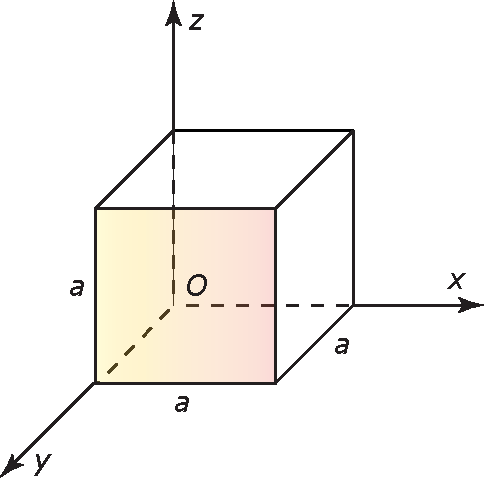
\includegraphics[width=0.25\linewidth]{fig/images/extension_cube.pdf}
  \caption{A cube of side length $a$ located with a vertex on the origin and the sides extending through the $x,y,z$ axes}
  \label{fig:extension_cube}
\end{figure}

We can immediately determine that:

\[\rho(x,y,z) = \rho\]
\[V = a^3\]
\[\rho = \frac{M}{a^3}\]

Our linearized integral results in:

\[\bm{I} = \iiint\limits_{V} \rho\left((x_k^2 + y_k^2 + z_k^2)\begin{bmatrix}1 & 0 & 0 \\ 0 & 1 & 0 \\ 0 & 0 & 1\end{bmatrix} - \begin{bmatrix}x_k \\ y_k \\ z_k\end{bmatrix} \otimes \begin{bmatrix}x_k \\ y_k \\ z_k\end{bmatrix}\right)dxdydz\]
\[\bm{I} = \iiint\limits_{V} \rho\left(\begin{bmatrix}x_k^2 + y_k^2 + z_k^2 & 0 & 0 \\ 0 & x_k^2 + y_k^2 + z_k^2 & 0 \\ 0 & 0 & x_k^2 + y_k^2 + z_k^2\end{bmatrix} - \begin{bmatrix}x_k^2 & x_ky_k & x_kz_k \\ x_ky_k & y_k^2 & y_kz_k \\ x_kz_k & y_kz_k & z_k^2 \end{bmatrix}\right)dxdydz\]
\[\bm{I} = \iiint\limits_{V} \rho\left(\begin{bmatrix}y_k^2 + z_k^2 & -x_ky_k & -x_kz_k \\ -x_ky_k & x_k^2 + z_k^2 & -y_kz_k \\ -x_kz_k & -y_kz_k & x_k^2 + y_k^2 \end{bmatrix}\right)dxdydz\]

The limits for our integrals simply span the length of the sides, or $0$ to $a$, transforming the problem into a multi-line integral in matrix form and allowing us to remove the $k$ subscripts defining each individual mass element:

\[\bm{I} = \rho\int_0^a \int_0^a \int_0^a  \left(\begin{bmatrix}y^2 + z^2 & -xy & -xz \\ -xy & x^2 + z^2 & -yz \\ -xz & -yz & x^2 + y^2 \end{bmatrix}\right)dxdydz\]

\[\bm{I} = \rho \int_0^a \int_0^a \int_0^a  \left(\begin{bmatrix}(y^2 + z^2)\left[x\right]_0^a & \left[\frac{-x^2y}{2}\right]_0^a & \left[\frac{-x^2z}{2}\right]_0^a \\ \left[\frac{-x^2y}{2}\right]_0^a & \left[\frac{x^3}{3} + xz^2\right]_0^a & \left[-xyz\right]_0^a \\ \left[\frac{-x^2z}{2}\right]_0^a & \left[-xyz\right]_0^a & \left[\frac{x^3}{3} + xy^2\right]_0^a \end{bmatrix}\right)dxdydz\]

\[\bm{I} = \rho \ \int_0^a \int_0^a  \left(\begin{bmatrix}ay^2 + az^2 & \frac{-a^2y}{2} & \frac{-a^2z}{2} \\ \frac{-a^2y}{2} & \frac{a^3}{3} + az^2 & -ayz \\ \frac{-a^2z}{2} & -ayz & \frac{a^3}{3} + ay^2 \end{bmatrix}\right)dydz\]

\[\bm{I} = \rho \ \int_0^a  \left(\begin{bmatrix}\left[\frac{ay^3}{3} + ayz^2\right]_0^a & \left[\frac{-a^2y^2}{4}\right]_0^a & \left[\frac{-a^2zy}{2}\right]_0^a \\ \left[\frac{-a^2y^2}{4}\right]_0^a & \left[\frac{a^3y}{3} + ayz^2\right]_0^a & \left[\frac{-ay^2z}{2}\right]_0^a \\ \left[\frac{-a^2zy}{2}\right]_0^a & \left[\frac{-ay^2z}{2}\right]_0^a & \left[\frac{a^3y}{3} + \frac{ay^3}{3}\right]_0^a \end{bmatrix}\right)dz\]

\[\bm{I} = \rho \ \int_0^a \left(\begin{bmatrix}\frac{a^4}{3} + a^2z^2 & \frac{-a^4}{4} & \frac{-a^3z}{2} \\ \frac{-a^4}{4} & \frac{a^4}{3} + a^2z^2 & \frac{-a^3z}{2} \\ \frac{-a^3z}{2} & \frac{-a^3z}{2} & \frac{2a^4}{3}\end{bmatrix}\right)dz\]


\[\bm{I} = \rho \begin{bmatrix} \left[\frac{a^4z}{3} + \frac{a^2z^3}{3}\right]_0^a & \left[\frac{-a^4z}{4}\right]_0^a & \left[\frac{-a^3z^2}{4}\right]_0^a \\ \left[\frac{-a^4z}{4}\right]_0^a & \left[\frac{a^4z}{3} + \frac{a^2z^3}{3}\right]_0^a & \left[\frac{-a^3z^2}{4}\right]_0^a \\ \left[\frac{-a^3z^2}{4}\right]_0^a & \left[\frac{-a^3z^2}{4}\right]_0^a & \left[\frac{2a^4z}{3}\right]_0^a \end{bmatrix}\]

Simplyifing, substituting for $\rho$, and reducing, results in a final moment of inertia tensor of:

\[\bm{I}_{\text{uniform cube}} =  \begin{bmatrix} \frac{2}{3}Ma^2 & -\frac{1}{4}Ma^2 & -\frac{1}{4}Ma^2 \\ -\frac{1}{4}Ma^2 & \frac{2}{3}Ma^2 & -\frac{1}{4}Ma^2 \\ -\frac{1}{4}Ma^2 & -\frac{1}{4}Ma^2 & \frac{2}{3}Ma^2\end{bmatrix}\]

We notice that the diagonal moment of inertia values ($I_{xx}, I_{yy}, I_{zz}$) are identical, as well as the off-diagonal values. This is somewhat intuitive because the cube has a uniform density and is situated symmetrically with respect to the individual axes. It is important to keep in mind that the moment of inertia is a measure of the difficulty of rotating a body about a given axis (much like inertia is the tendency of a body to resist translational motion), so this matrix allows us to easily determine the angular momentum or energy of a body rotating about any axis passing through the origin (as this was the assumed reference point). To calculate the moment of inertia about any axis passing through the reference point, we can simply use the relation described in \cref{eq:matrix_to_moment}, where $\bm{\hat{\omega}}$ represents the unit angular velocity vector for a given axis of rotation~\parencite{Kreyszig_Kreyszig_Norminton_2011}. 

\begin{equation}
I = \bm{\hat{\omega}}^T\bm{I}\bm{\hat{\omega}}
\label{eq:matrix_to_moment}
\end{equation}

The proof for this result is left out, as it is outside the scope of the investigation, but the equation can be used to quickly determine the moment of inertia for the cube about its diagonal, something which was difficult to do using traditional methods. The unit vector for this diagonal axis is simply $\begin{bmatrix}\frac{1}{\sqrt{3}} \\ \frac{1}{\sqrt{3}} \\ \frac{1}{\sqrt{3}}\end{bmatrix}$, so:

\[I = \begin{bmatrix}\frac{1}{\sqrt{3}} & \frac{1}{\sqrt{3}} & \frac{1}{\sqrt{3}}\end{bmatrix}\begin{bmatrix} \frac{2}{3}Ma^2 & -\frac{1}{4}Ma^2 & -\frac{1}{4}Ma^2 \\ -\frac{1}{4}Ma^2 & \frac{2}{3}Ma^2 & -\frac{1}{4}Ma^2 \\ -\frac{1}{4}Ma^2 & -\frac{1}{4}Ma^2 & \frac{2}{3}Ma^2\end{bmatrix}\begin{bmatrix}\frac{1}{\sqrt{3}} \\ \frac{1}{\sqrt{3}} \\ \frac{1}{\sqrt{3}}\end{bmatrix} = \begin{bmatrix}\frac{1}{6\sqrt{3}}Ma^2 & \frac{1}{6\sqrt{3}}Ma^2 & \frac{1}{6\sqrt{3}}Ma^2\end{bmatrix}\begin{bmatrix}\frac{1}{\sqrt{3}} \\ \frac{1}{\sqrt{3}} \\ \frac{1}{\sqrt{3}}\end{bmatrix} = \frac{1}{6}Ma^2\] 

In this simple manner, the moment of inertia can easily be calculated for any potential axis, and the entire approach can easily be adopted for other bodies, not only cubes. This matrix can also be shifted in order to make the center of mass and reference point coincide, which eliminates the off-diagonal values entirely and results in a matrix with only 3 defining values.